\documentclass[12pt,a4paper]{report}
\usepackage[T1]{fontenc}
\usepackage{lmodern}
\usepackage{anyfontsize}
\usepackage[a4paper, top=1in, bottom=1in, left=1in, right=1in]{geometry}
\usepackage{graphicx}
\usepackage{setspace}
\usepackage{titlesec}
\usepackage{ragged2e}
\usepackage{enumitem}
\usepackage{tikz}
\usepackage{longtable}
\usepackage{array}
\usepackage{booktabs}
\usepackage{hyperref}
\usepackage{xcolor}
\usepackage{float}
\usepackage{caption}
\usepackage{subcaption}
\usepackage{fancyhdr}
\usepackage{pgfplots}
\pgfplotsset{compat=1.18}

\usetikzlibrary{shapes.geometric, arrows.meta, positioning, calc, fit, backgrounds}

% Color definitions
\definecolor{primaryblue}{HTML}{6366F1}
\definecolor{accentcyan}{HTML}{06B6D4}
\definecolor{darkbg}{HTML}{0A0B14}
\definecolor{cardbg}{HTML}{13162B}
\definecolor{bordercolor}{HTML}{252840}
\definecolor{textmuted}{HTML}{5C6385}
\definecolor{successgreen}{HTML}{22C55E}
\definecolor{warningamber}{HTML}{F59E0B}
\definecolor{errorred}{HTML}{EF4444}

\setstretch{1.15}
\setlength{\parskip}{6pt}
\setlength{\parindent}{0pt}
\setlist[enumerate]{itemsep=6pt, parsep=0pt, topsep=8pt, partopsep=0pt, leftmargin=1cm}
\setlist[itemize]{itemsep=4pt, parsep=0pt, topsep=6pt, partopsep=0pt, leftmargin=1.2cm}

\hypersetup{
  colorlinks=true,
  linkcolor=black,
  urlcolor=black,
  citecolor=black,
}

% Header/Footer
\pagestyle{fancy}
\fancyhf{}
\fancyhead[L]{\small\textcolor{textmuted}{Academic Status Transparency Notification System -- Midterm Report}}
\fancyhead[R]{\small\textcolor{textmuted}{Group G14}}
\fancyfoot[C]{\thepage}
\renewcommand{\headrulewidth}{0.4pt}

\begin{document}

%% ===========================
%% TITLE PAGE
%% ===========================
\begin{titlepage}
\centering
\vspace*{1cm}

{\Large \textbf{A Midterm Progress Report}}\\[0.5cm]
{\Large \textbf{on}}\\[0.5cm]
{\fontsize{24}{28}\selectfont \textbf{Academic Status}}\\[0.15cm]
{\fontsize{24}{28}\selectfont \textbf{Transparency Notification System}}\\[0.8cm]

{\fontsize{12}{14}\selectfont \textbf{Submitted in partial fulfillment of the requirements for the award of the degree of}}\\[1cm]

{\fontsize{14}{16}\selectfont \textbf{BACHELOR OF TECHNOLOGY}}\\[0.3cm]
{\fontsize{14}{16}\selectfont Computer Science \& Engineering}\\[1cm]

SUBMITTED BY\\[0.8cm]

\begin{center}
\begin{minipage}[t]{0.3\textwidth}
\centering
{\fontsize{13}{15}\selectfont ARSHDEEP ANAND}\\[0.1cm]
{\fontsize{11}{13}\selectfont URN: 2302481}\\[0.1cm]
{\fontsize{11}{13}\selectfont CRN: 2315025}
\end{minipage}
\hfill
\begin{minipage}[t]{0.3\textwidth}
\centering
{\fontsize{13}{15}\selectfont NISHTHA JAIN}\\[0.1cm]
{\fontsize{11}{13}\selectfont URN: 2302627}\\[0.1cm]
{\fontsize{11}{13}\selectfont CRN: 2315172}
\end{minipage}
\hfill
\begin{minipage}[t]{0.3\textwidth}
\centering
{\fontsize{13}{15}\selectfont BALKRISHAN SINGH}\\[0.1cm]
{\fontsize{11}{13}\selectfont URN: 2302492}\\[0.1cm]
{\fontsize{11}{13}\selectfont CRN: 2315036}
\end{minipage}
\vspace{0.8cm}

{\fontsize{14}{16}\selectfont UNDER THE GUIDANCE OF}\\[0.15cm]
{\fontsize{14}{16}\selectfont Dr. Kapil Sharma}\\[0.15cm]
\end{center}

\vspace{0.8cm}
\begin{center}
\includegraphics[height=3.5cm]{assets/image.png}
\end{center}
\vspace{0.8cm}

{\bfseries \Large Department of Computer Science and Engineering}\\[0.3cm]
{\fontsize{16}{18}\selectfont \textbf{GURU NANAK DEV ENGINEERING COLLEGE,}}\\[0.3cm]
{\fontsize{16}{18}\selectfont \textbf{LUDHIANA}}\\

\vfill
\end{titlepage}

%% ===========================
%% TABLE OF CONTENTS
%% ===========================
\tableofcontents
\newpage

%% ===========================
%% CHAPTER 1: INTRODUCTION
%% ===========================
\chapter{Introduction}

\section{Project Overview}

The \textbf{Academic Status Transparency Notification System} (hereafter referred to as \textbf{ASTNS}) is a full-stack web application designed to bridge the communication gap between academic institutions and parents/guardians of students. The system provides a transparent mechanism for notifying guardians about a student's academic performance, including semester-wise marks, SGPA/CGPA tracking, and detention status, thereby fostering timely parental intervention.

In many educational institutions, academic performance data remains confined within the campus boundaries. Guardians often learn about their ward's academic difficulties only at the end of the academic year. ASTNS addresses this by providing:

\begin{itemize}
  \item \textbf{Real-time academic transparency} -- Guardians receive automated email notifications with secure, tokenised links to view their ward's detailed semester report.
  \item \textbf{Centralised admin dashboard} -- Administrators can upload academic records in bulk (CSV/Excel), manage student data, dispatch notifications, and monitor access tokens from a single panel.
  \item \textbf{Guardian portal} -- Guardians access a read-only, visually rich dashboard showing semester-wise marks, SGPA trends via interactive charts, detention alerts, and attendance data.
\end{itemize}

\section{Objectives}

\begin{enumerate}
  \item To design and develop a web-based Academic Status Transparency Notification System that enables administrators to upload student academic data in bulk via CSV/Excel formats.
  \item To automatically notify guardians via email with secure, time-limited access links, providing a Guardian Dashboard for viewing detailed semester reports with visual analytics.
  \item To implement a Token Management system ensuring secure, traceable access to student records.
\end{enumerate}

\section{Scope of the Project}

The system is designed for use by engineering colleges affiliated with I.K. Gujral Punjab Technical University (IKGPTU). It supports multiple courses (B.Tech, M.Tech, MBA, MCA, BCA, B.Arch, B.Voc., B.Com, BBA) and their respective branches. The scope includes:

\begin{itemize}
  \item Admin authentication and session management.
  \item Bulk data upload and validation.
  \item Email notification dispatch via SMTP (Gmail).
  \item Token-based guardian access with expiry and revocation.
  \item Interactive data visualisation using charts.
  \item Serverless deployment on Vercel.
\end{itemize}

%% ===========================
%% CHAPTER 2: SYSTEM REQUIREMENTS
%% ===========================
\chapter{System Requirements}

\section{Software Requirements}

\begin{longtable}{|p{4cm}|p{4.5cm}|p{4.5cm}|}
\hline
\textbf{Category} & \textbf{Technology} & \textbf{Version / Details}\\
\hline
\endfirsthead
\hline
\textbf{Category} & \textbf{Technology} & \textbf{Version / Details}\\
\hline
\endhead
Runtime & Node.js & v20+ (LTS)\\
\hline
Frontend Framework & React & 19.2.0\\
\hline
Build Tool & Vite & 7.3.1\\
\hline
CSS Framework & Tailwind CSS & 4.2.1\\
\hline
Charts Library & Recharts & 3.7.0\\
\hline
Form Management & React Hook Form & 7.71.2\\
\hline
Routing & React Router DOM & 7.13.1\\
\hline
Icons & Lucide React & 0.575.0\\
\hline
HTTP Client & Axios & 1.13.6\\
\hline
Backend Framework & Express.js & 5.2.1\\
\hline
Database & MongoDB Atlas & M0 Free Tier\\
\hline
ODM & Mongoose & 9.2.3\\
\hline
Email Service & Nodemailer & 8.0.1\\
\hline
Deployment & Vercel & Serverless Functions\\
\hline
Version Control & Git + GitHub & Latest\\
\hline
IDE & VS Code & Latest\\
\hline
Browser & Chrome / Arc & Latest\\
\hline
OS & macOS / Windows & Development\\
\hline
\end{longtable}

\clearpage
\section{Hardware Requirements}

\begin{longtable}{|p{3cm}|p{9cm}|}
\hline
\textbf{Component} & \textbf{Minimum Specification}\\
\hline
\endfirsthead
Processor & Intel i5 / Apple M1 or equivalent\\
\hline
RAM & 8 GB (minimum)\\
\hline
Storage & 256 GB SSD\\
\hline
Internet & Broadband (for MongoDB Atlas, SMTP, Vercel)\\
\hline
Display & 1366 $\times$ 768 resolution or higher\\
\hline
\end{longtable}

%% ===========================
%% CHAPTER 3: SOFTWARE REQUIREMENT ANALYSIS
%% ===========================
\chapter{Software Requirement Analysis}

\section{Problem Definition}

In the current academic ecosystem, parents and guardians of college students often lack timely access to their ward's academic performance data. Results are published on university portals, but guardians may not be aware of:
\begin{itemize}
  \item Detention in internal or external examinations.
  \item Declining SGPA trends across semesters.
  \item Subject-wise performance breakdowns.
\end{itemize}

This communication gap delays corrective intervention, potentially resulting in academic backlogs. ASTNS solves this by automating the notification pipeline.

\section{Module Definitions}

The system is divided into the following functional modules:

\begin{figure}[H]
\centering
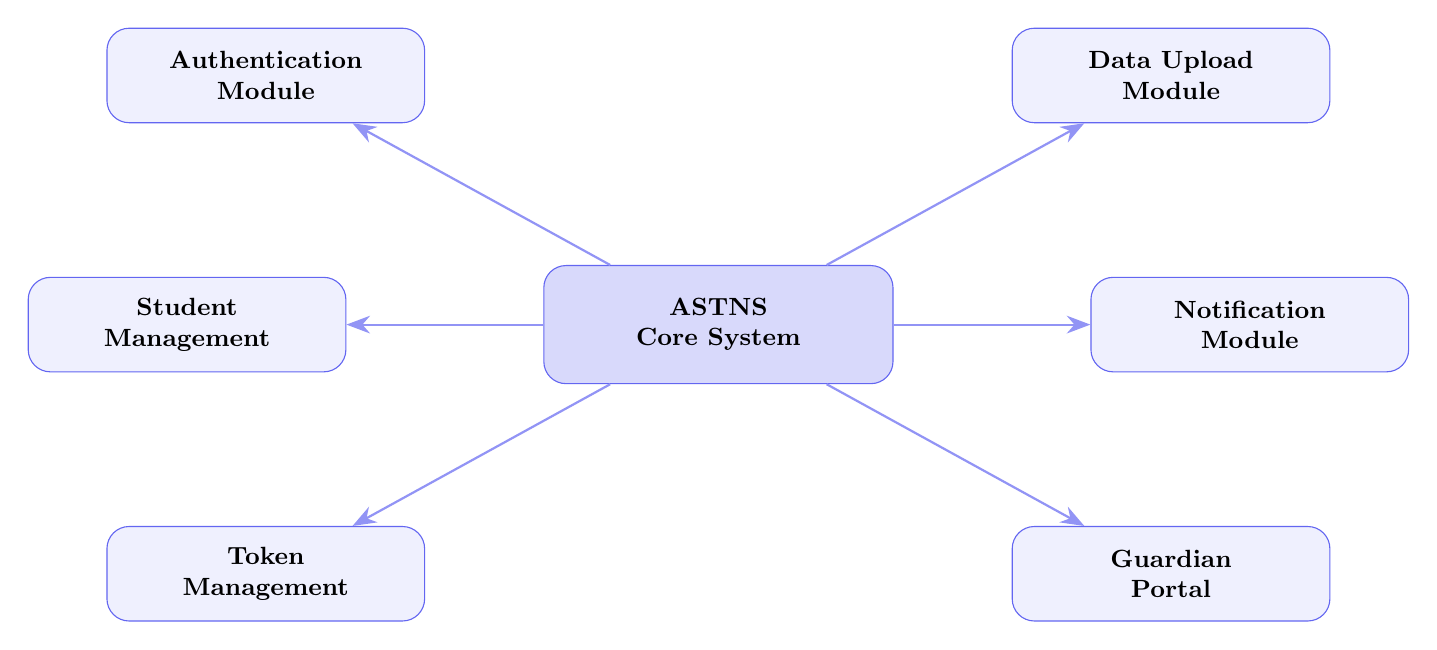
\begin{tikzpicture}[
  module/.style={rectangle, draw=primaryblue, fill=primaryblue!10, rounded corners=8pt, text width=3.8cm, minimum height=1.2cm, align=center, font=\small\bfseries},
  arrow/.style={-{Stealth[length=3mm]}, thick, draw=primaryblue!70}
]
  % Central node
  \node[module, fill=primaryblue!25, text width=4.2cm, minimum height=1.5cm] (core) {ASTNS\\Core System};

  % Modules
  \node[module, above left=1.8cm and 1.5cm of core] (auth) {Authentication\\Module};
  \node[module, above right=1.8cm and 1.5cm of core] (upload) {Data Upload\\Module};
  \node[module, left=2.5cm of core] (student) {Student\\Management};
  \node[module, right=2.5cm of core] (notify) {Notification\\Module};
  \node[module, below left=1.8cm and 1.5cm of core] (token) {Token\\Management};
  \node[module, below right=1.8cm and 1.5cm of core] (guardian) {Guardian\\Portal};

  % Arrows
  \draw[arrow] (core) -- (auth);
  \draw[arrow] (core) -- (upload);
  \draw[arrow] (core) -- (student);
  \draw[arrow] (core) -- (notify);
  \draw[arrow] (core) -- (token);
  \draw[arrow] (core) -- (guardian);
\end{tikzpicture}
\caption{System Module Architecture}
\end{figure}

\subsection{Module 1: Authentication Module}
\begin{itemize}
  \item Admin login with email/password verification.
  \item Form validation using React Hook Form with real-time error feedback.
  \item Session management and route protection.
\end{itemize}

\subsection{Module 2: Data Upload Module}
\begin{itemize}
  \item Accepts CSV and Excel files for bulk student data import.
  \item Drag-and-drop interface with file type validation.
  \item Course and branch selection with dynamic dropdown mapping.
  \item Preview of parsed records before submission.
\end{itemize}

\subsection{Module 3: Student Management Module}
\begin{itemize}
  \item Searchable student list with grid/list view toggle.
  \item Filters by branch, semester, and SGPA range.
  \item Detailed student profile with semester-wise mark breakdown.
  \item Interactive SGPA trend chart (LineChart via Recharts).
  \item Detention status highlighting.
\end{itemize}

\subsection{Module 4: Notification Module}
\begin{itemize}
  \item Multi-select students for batch notification dispatch.
  \item Email notification via Nodemailer (Gmail SMTP).
  \item HTML email template with branded ``View Report'' button.
  \item Dynamic URL generation with unique student identifier.
\end{itemize}

\subsection{Module 5: Token Management Module}
\begin{itemize}
  \item Tracks all generated access tokens.
  \item Display of token status (Active, Expired, Revoked).
  \item One-click token revocation and link copying.
  \item Access method tracking (Email, WhatsApp, Direct).
\end{itemize}

\subsection{Module 6: Guardian Portal}
\begin{itemize}
  \item Token-based secure access (no login required).
  \item Student profile with academic summary.
  \item Semester-wise collapsible mark tables with pass/detained indicators.
  \item Interactive SGPA trend line chart.
  \item Attendance ring indicator using SVG.
  \item Report download functionality.
\end{itemize}

%% ===========================
%% CHAPTER 4: SOFTWARE DESIGN
%% ===========================
\chapter{Software Design}

\section{System Architecture -- Block Diagram}

\begin{figure}[H]
\centering
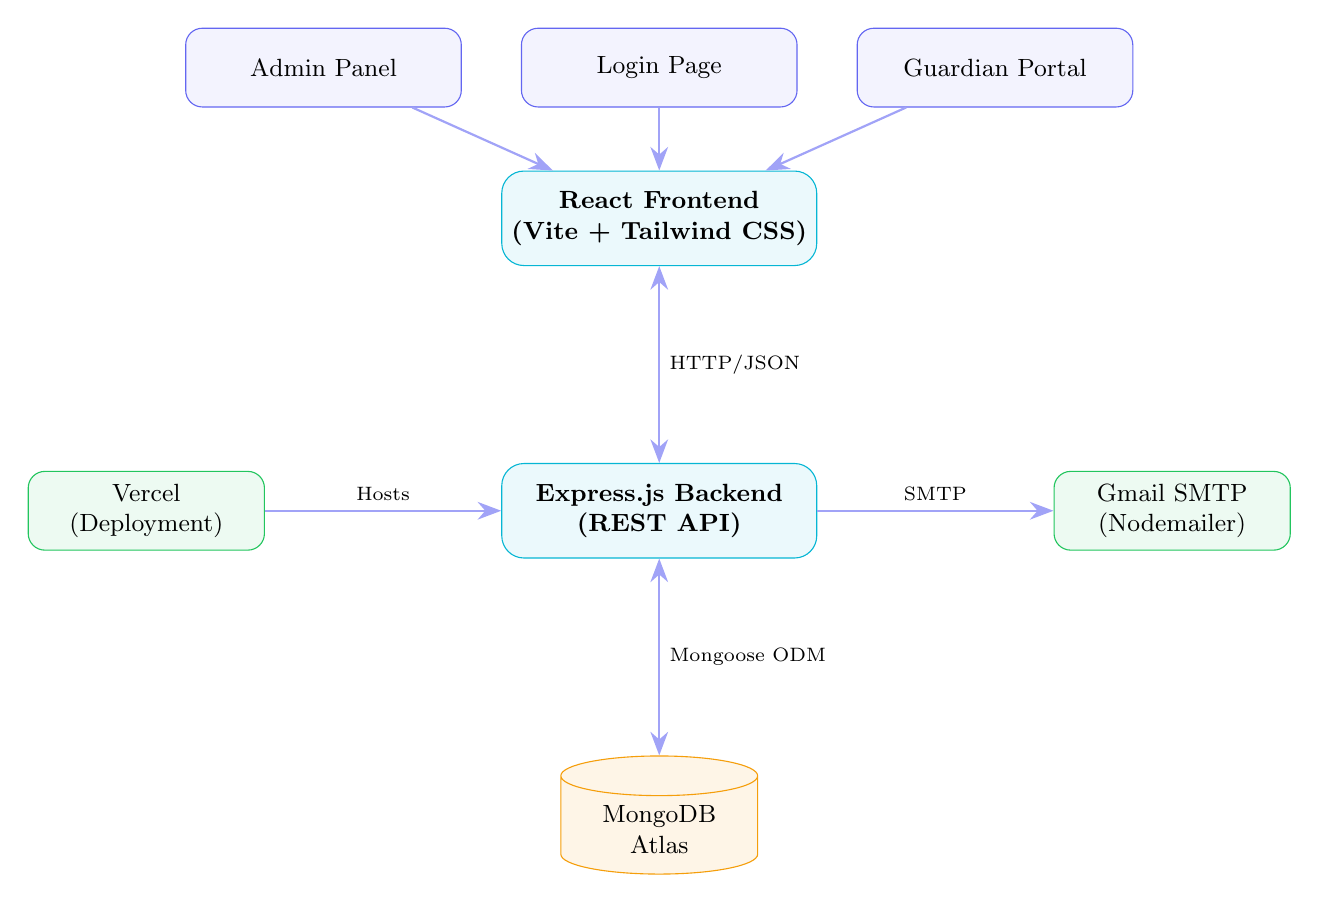
\begin{tikzpicture}[
  block/.style={rectangle, draw=primaryblue, fill=primaryblue!8, rounded corners=6pt, minimum width=3.5cm, minimum height=1cm, align=center, font=\small},
  bigblock/.style={rectangle, draw=accentcyan, fill=accentcyan!8, rounded corners=8pt, minimum width=4cm, minimum height=1.2cm, align=center, font=\small\bfseries},
  dbblock/.style={cylinder, draw=warningamber, fill=warningamber!10, shape border rotate=90, minimum width=2.5cm, minimum height=1.5cm, aspect=0.3, align=center, font=\small},
  extblock/.style={rectangle, draw=successgreen, fill=successgreen!8, rounded corners=6pt, minimum width=3cm, minimum height=1cm, align=center, font=\small},
  arrow/.style={-{Stealth[length=3mm]}, thick, draw=primaryblue!60},
  darrow/.style={{Stealth[length=3mm]}-{Stealth[length=3mm]}, thick, draw=primaryblue!60}
]
  % Frontend
  \node[bigblock] (frontend) {React Frontend\\(Vite + Tailwind CSS)};

  % Backend
  \node[bigblock, below=2.5cm of frontend] (backend) {Express.js Backend\\(REST API)};

  % Database
  \node[dbblock, below=2.5cm of backend] (db) {MongoDB\\Atlas};

  % External Services
  \node[extblock, right=3cm of backend] (email) {Gmail SMTP\\(Nodemailer)};
  \node[extblock, left=3cm of backend] (vercel) {Vercel\\(Deployment)};

  % Sub-components of frontend
  \node[block, above left=0.8cm and 0.5cm of frontend]  (admin)    {Admin Panel};
  \node[block, above right=0.8cm and 0.5cm of frontend] (guardian)  {Guardian Portal};
  \node[block, above=0.8cm of frontend]                 (login)    {Login Page};

  % Arrows
  \draw[arrow] (admin) -- (frontend);
  \draw[arrow] (guardian) -- (frontend);
  \draw[arrow] (login) -- (frontend);
  \draw[darrow] (frontend) -- node[right, font=\scriptsize]  {HTTP/JSON} (backend);
  \draw[darrow] (backend) -- node[right, font=\scriptsize]  {Mongoose ODM} (db);
  \draw[arrow] (backend) -- node[above, font=\scriptsize]  {SMTP} (email);
  \draw[arrow] (vercel) -- node[above, font=\scriptsize]  {Hosts} (backend);
\end{tikzpicture}
\caption{System Architecture Block Diagram}
\end{figure}

The System Architecture Block Diagram (Figure 4.1) outlines the high-level components of the system. It illustrates how the React-based frontend interfaces with the Express.js backend via HTTP/REST APIs. The backend then communicates seamlessly with the MongoDB Atlas database for data persistence and the Gmail SMTP server for dispatching notifications. Vercel acts as the overarching cloud hosting environment for both the frontend SPA and backend serverless functions.

\section{Data Flow Diagram (DFD)}

\subsection{Level 0 -- Context Diagram}

\begin{figure}[H]
\centering
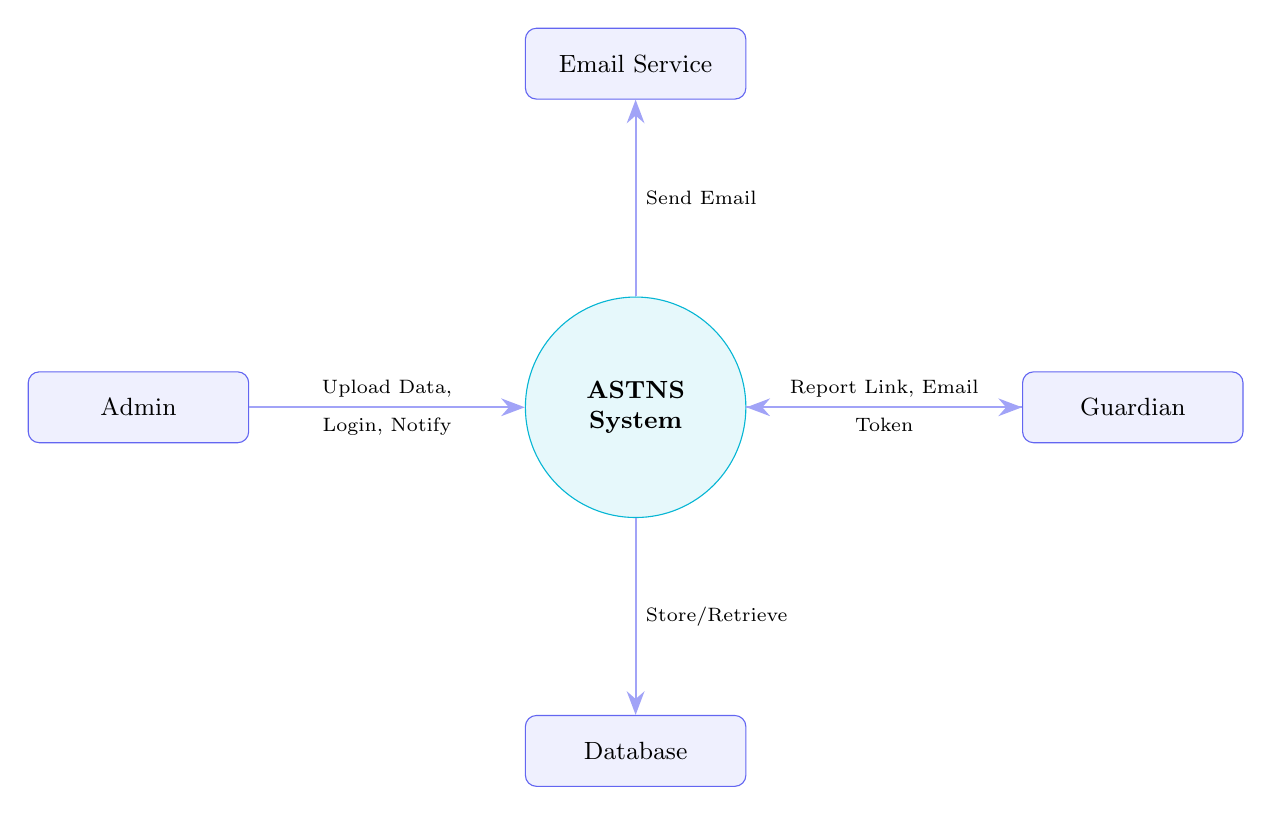
\begin{tikzpicture}[
  entity/.style={rectangle, draw=primaryblue, fill=primaryblue!10, rounded corners=4pt, minimum width=2.8cm, minimum height=0.9cm, align=center, font=\small},
  process/.style={circle, draw=accentcyan, fill=accentcyan!10, minimum size=2.8cm, align=center, font=\small\bfseries},
  arrow/.style={-{Stealth[length=3mm]}, thick, draw=primaryblue!60}
]
  \node[process] (sys) {ASTNS\\System};
  \node[entity, left=3.5cm of sys] (admin) {Admin};
  \node[entity, right=3.5cm of sys] (guardian) {Guardian};
  \node[entity, below=2.5cm of sys] (db) {Database};
  \node[entity, above=2.5cm of sys] (email) {Email Service};

  \draw[arrow] (admin) -- node[above, font=\scriptsize] {Upload Data,} node[below, font=\scriptsize] {Login, Notify} (sys);
  \draw[arrow] (sys) -- node[above, font=\scriptsize] {Report Link, Email} (guardian);
  \draw[arrow] (guardian) -- node[below, font=\scriptsize, sloped] {Token} (sys);
  \draw[arrow] (sys) -- node[right, font=\scriptsize] {Store/Retrieve} (db);
  \draw[arrow] (sys) -- node[right, font=\scriptsize] {Send Email} (email);
\end{tikzpicture}
\caption{Level 0 DFD -- Context Diagram}
\end{figure}

The Level 0 Context Diagram (Figure 4.2) presents the entire application as a single high-level process, highlighting its interactions with external entities. The Admin provides academic data and triggers notifications, while the Guardian receives the notification email and subsequently uses a secure token to access the generated report. The core system interfaces heavily with the external Database and Email Service to fulfill these requests.

\subsection{Level 1 -- DFD}

\begin{figure}[H]
\centering
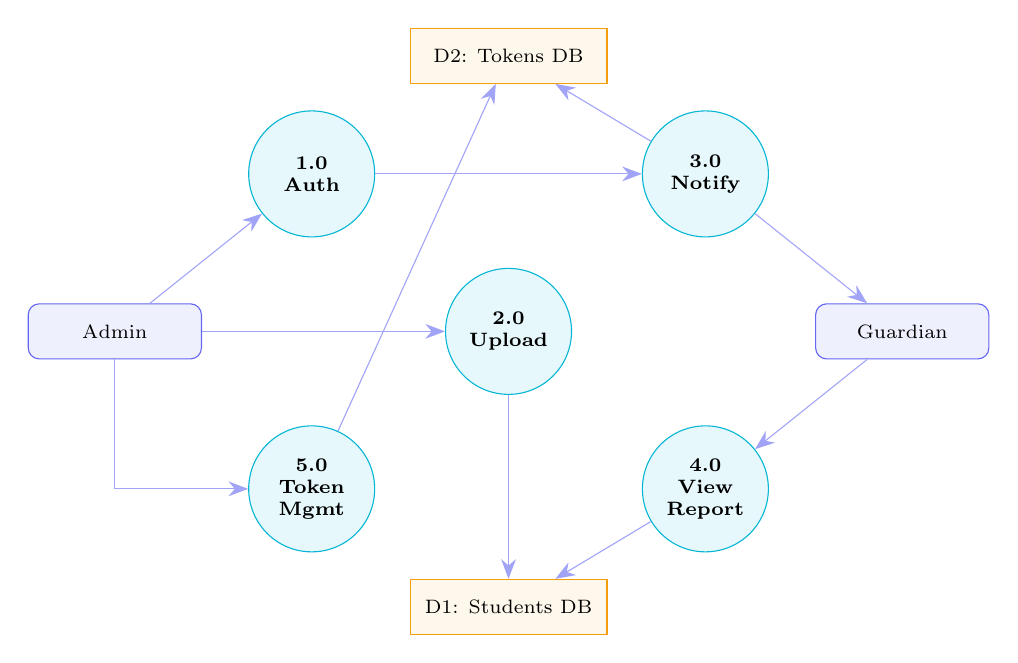
\begin{tikzpicture}[
  entity/.style={rectangle, draw=primaryblue, fill=primaryblue!10, rounded corners=4pt, minimum width=2.2cm, minimum height=0.7cm, align=center, font=\scriptsize},
  process/.style={circle, draw=accentcyan, fill=accentcyan!10, minimum size=1.6cm, align=center, font=\scriptsize\bfseries},
  store/.style={rectangle, draw=warningamber, fill=warningamber!8, minimum width=2.5cm, minimum height=0.7cm, align=center, font=\scriptsize},
  arrow/.style={-{Stealth[length=2.5mm]}, draw=primaryblue!60}
]
  % Entities
  \node[entity] (admin) at (-5,0) {Admin};
  \node[entity] (guardian) at (5,0) {Guardian};

  % Processes
  \node[process] (p1) at (-2.5, 2) {1.0\\Auth};
  \node[process] (p2) at (0, 0) {2.0\\Upload};
  \node[process] (p3) at (2.5, 2) {3.0\\Notify};
  \node[process] (p4) at (2.5, -2) {4.0\\View\\Report};
  \node[process] (p5) at (-2.5, -2) {5.0\\Token\\Mgmt};

  % Data stores
  \node[store] (ds1) at (0, -3.5) {D1: Students DB};
  \node[store] (ds2) at (0, 3.5) {D2: Tokens DB};

  % Arrows
  \draw[arrow] (admin) -- (p1);
  \draw[arrow] (admin) -- (p2);
  \draw[arrow] (p2) -- (ds1);
  \draw[arrow] (p3) -- (guardian);
  \draw[arrow] (guardian) -- (p4);
  \draw[arrow] (p4) -- (ds1);
  \draw[arrow] (p3) -- (ds2);
  \draw[arrow] (p5) -- (ds2);
  \draw[arrow] (admin) |- (p5);
  \draw[arrow] (p1) -- (p3);
\end{tikzpicture}
\caption{Level 1 DFD}
\end{figure}

The Level 1 Data Flow Diagram (Figure 4.3) breaks down the main system into granular sub-processes. It traces the flow of data starting from the Admin authenticating (1.0) and uploading academic records (2.0) into the Students DB. It further delineates the notification process (3.0), where secure tokens are generated and stored, followed by the Guardian providing the token to view the academic report (4.0).

\section{Use Case Diagram}

\begin{figure}[H]
\centering
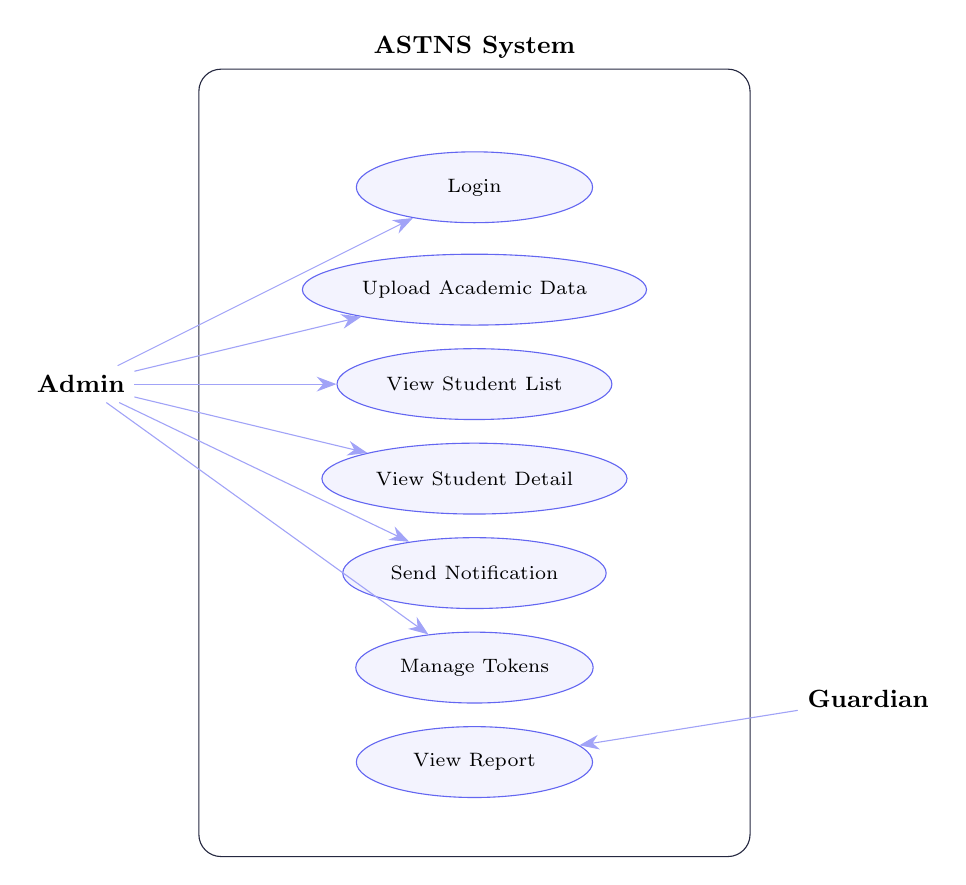
\begin{tikzpicture}[
  actor/.style={font=\small},
  usecase/.style={ellipse, draw=primaryblue, fill=primaryblue!8, minimum width=3cm, minimum height=0.9cm, align=center, font=\scriptsize},
  arrow/.style={-{Stealth[length=2.5mm]}, draw=primaryblue!60},
  sysbox/.style={rectangle, draw=bordercolor, rounded corners=8pt, minimum width=7cm, minimum height=10cm}
]
  % System boundary
  \node[sysbox, label={[font=\small\bfseries]above:ASTNS System}] (sys) at (0,0) {};

  % Use cases
  \node[usecase] (uc1) at (0, 3.5)  {Login};
  \node[usecase] (uc2) at (0, 2.2)  {Upload Academic Data};
  \node[usecase] (uc3) at (0, 1.0)  {View Student List};
  \node[usecase] (uc4) at (0, -0.2) {View Student Detail};
  \node[usecase] (uc5) at (0, -1.4) {Send Notification};
  \node[usecase] (uc6) at (0, -2.6) {Manage Tokens};
  \node[usecase] (uc7) at (0, -3.8) {View Report};

  % Actors
  \node[actor] (adm) at (-5, 1.0) {\textbf{Admin}};
  \node[actor] (grd) at (5, -3.0)  {\textbf{Guardian}};

  % Admin connections
  \draw[arrow] (adm) -- (uc1);
  \draw[arrow] (adm) -- (uc2);
  \draw[arrow] (adm) -- (uc3);
  \draw[arrow] (adm) -- (uc4);
  \draw[arrow] (adm) -- (uc5);
  \draw[arrow] (adm) -- (uc6);

  % Guardian connections
  \draw[arrow] (grd) -- (uc7);
\end{tikzpicture}
\caption{Use Case Diagram}
\end{figure}

The Use Case Diagram (Figure 4.4) illustrates the primary interactions between the actors and the system. The Admin is responsible for managing the system through authentication, uploading academic data, viewing student lists and details, dispatching notifications, and managing access tokens. Conversely, the Guardian has a focused interaction limited to viewing the generated academic report via a secure token without needing a traditional login account.

\section{Sequence Diagram -- Notification Flow}

\begin{figure}[H]
\centering
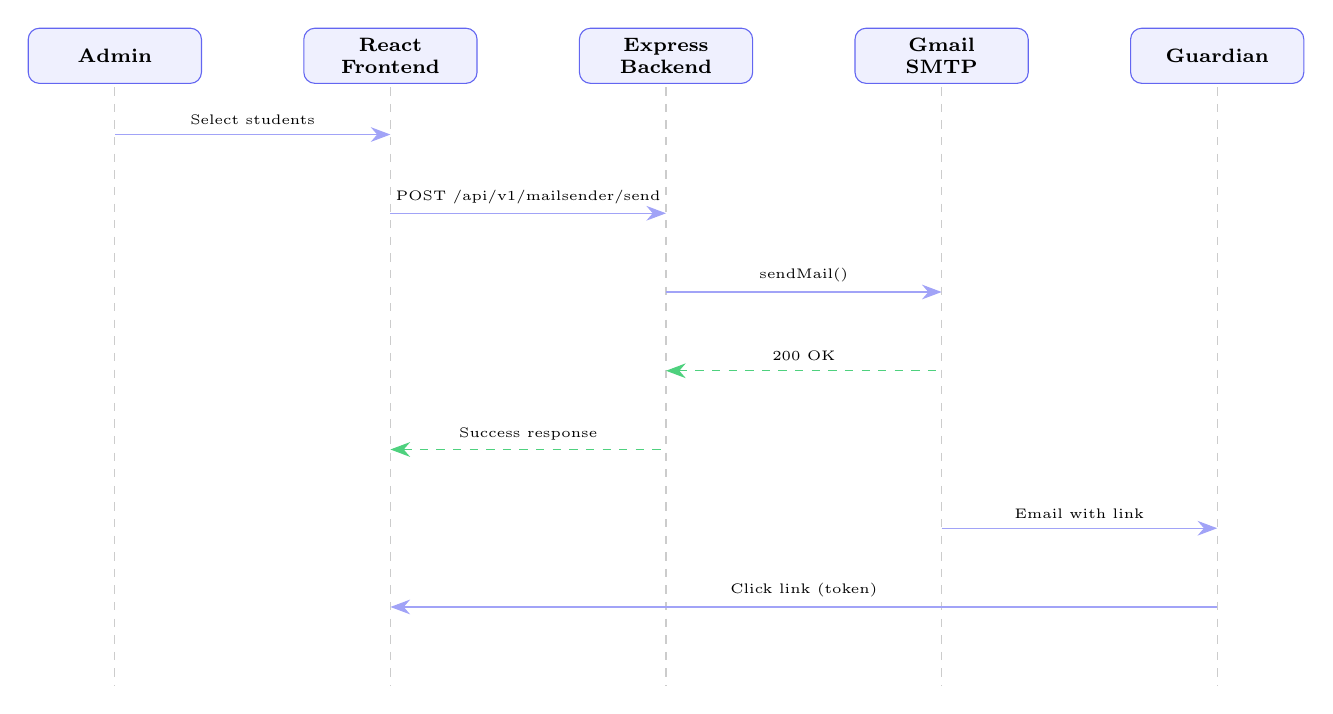
\begin{tikzpicture}[
  box/.style={rectangle, draw=primaryblue, fill=primaryblue!10, rounded corners=4pt, minimum width=2.2cm, minimum height=0.7cm, align=center, font=\scriptsize\bfseries},
  arrow/.style={-{Stealth[length=2.5mm]}, draw=primaryblue!60},
  darrow/.style={{Stealth[length=2.5mm]}-, draw=successgreen!80, dashed}
]
  % Lifelines
  \node[box] (admin) at (0, 0) {Admin};
  \node[box] (frontend) at (3.5, 0) {React\\Frontend};
  \node[box] (backend) at (7, 0) {Express\\Backend};
  \node[box] (smtp) at (10.5, 0) {Gmail\\SMTP};
  \node[box] (guardian) at (14, 0) {Guardian};

  % Lifelines
  \draw[dashed, gray!40] (0, -0.4) -- (0, -8);
  \draw[dashed, gray!40] (3.5, -0.4) -- (3.5, -8);
  \draw[dashed, gray!40] (7, -0.4) -- (7, -8);
  \draw[dashed, gray!40] (10.5, -0.4) -- (10.5, -8);
  \draw[dashed, gray!40] (14, -0.4) -- (14, -8);

  % Messages
  \draw[arrow] (0, -1) -- node[above, font=\tiny] {Select students} (3.5, -1);
  \draw[arrow] (3.5, -2) -- node[above, font=\tiny] {POST /api/v1/mailsender/send} (7, -2);
  \draw[arrow] (7, -3) -- node[above, font=\tiny] {sendMail()} (10.5, -3);
  \draw[darrow] (7, -4) -- node[above, font=\tiny] {200 OK} (10.5, -4);
  \draw[darrow] (3.5, -5) -- node[above, font=\tiny] {Success response} (7, -5);
  \draw[arrow] (10.5, -6) -- node[above, font=\tiny] {Email with link} (14, -6);
  \draw[arrow] (14, -7) -- node[above, font=\tiny] {Click link (token)} (3.5, -7);
\end{tikzpicture}
\caption{Sequence Diagram -- Notification Flow}
\end{figure}

The Sequence Diagram (Figure 4.5) details the chronological flow of messages during the notification dispatch process. It shows the Admin initiating the process from the React Frontend by selecting students, which then sends a POST request to the Express Backend. The backend invokes the Gmail SMTP service to deliver an email with a secure link to the Guardian. Finally, the Guardian clicks the link, passing the token back to the frontend to access the report.

\section{Activity Diagram -- Admin Workflow}

\begin{figure}[H]
\centering
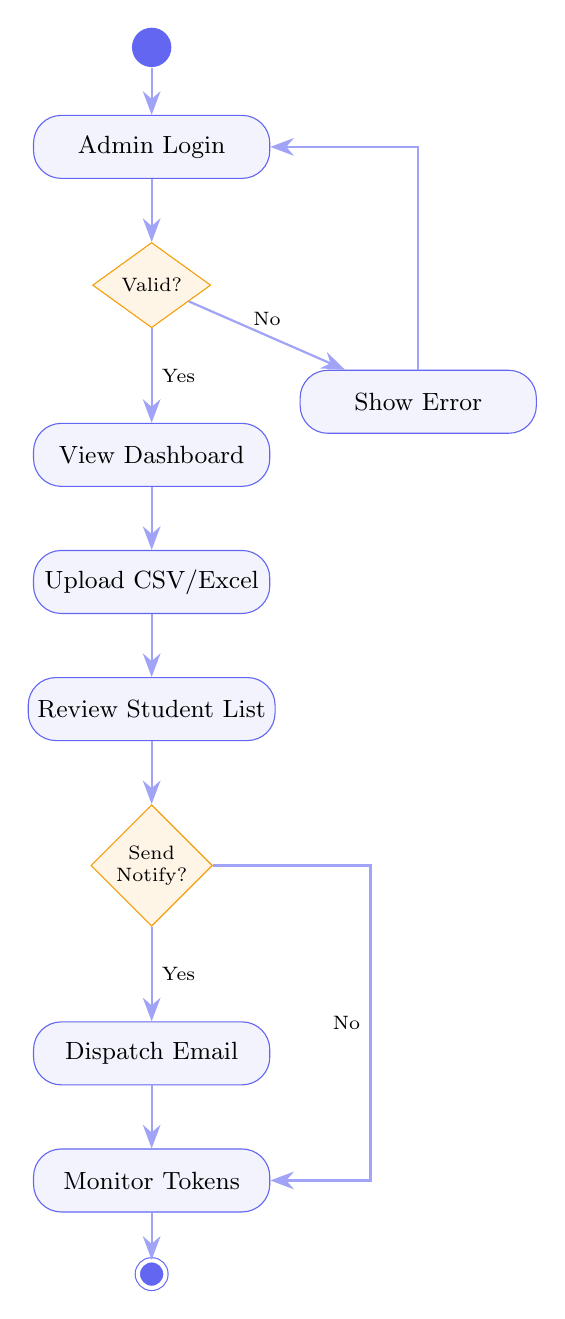
\begin{tikzpicture}[
  start/.style={circle, fill=primaryblue, minimum size=0.5cm},
  stop/.style={circle, draw=primaryblue, fill=primaryblue, minimum size=0.35cm, double, double distance=1.5pt},
  activity/.style={rectangle, draw=primaryblue, fill=primaryblue!8, rounded corners=10pt, minimum width=3cm, minimum height=0.8cm, align=center, font=\small},
  decision/.style={diamond, draw=warningamber, fill=warningamber!10, minimum width=1.5cm, minimum height=1cm, align=center, font=\scriptsize, inner sep=1pt},
  arrow/.style={-{Stealth[length=3mm]}, thick, draw=primaryblue!60}
]
  \node[start] (s) at (0, 0) {};
  \node[activity, below=0.6cm of s] (login) {Admin Login};
  \node[decision, below=0.8cm of login] (d1) {Valid?};
  \node[activity, below right=0.8cm and 1.5cm of d1] (err) {Show Error};
  \node[activity, below=1.2cm of d1] (dash) {View Dashboard};
  \node[activity, below=0.8cm of dash] (upload) {Upload CSV/Excel};
  \node[activity, below=0.8cm of upload] (review) {Review Student List};
  \node[decision, below=0.8cm of review] (d2) {Send\\Notify?};
  \node[activity, below=1.2cm of d2] (notify) {Dispatch Email};
  \node[activity, below=0.8cm of notify] (token) {Monitor Tokens};
  \node[stop, below=0.6cm of token] (e) {};

  \draw[arrow] (s) -- (login);
  \draw[arrow] (login) -- (d1);
  \draw[arrow] (d1) -- node[right, font=\scriptsize] {Yes} (dash);
  \draw[arrow] (d1) -- node[above, font=\scriptsize] {No} (err);
  \draw[arrow] (err) |- (login);
  \draw[arrow] (dash) -- (upload);
  \draw[arrow] (upload) -- (review);
  \draw[arrow] (review) -- (d2);
  \draw[arrow] (d2) -- node[right, font=\scriptsize] {Yes} (notify);
  \draw[arrow] (d2.east) -| ++(2, 0) |- node[left, font=\scriptsize, near start] {No} (token);
  \draw[arrow] (notify) -- (token);
  \draw[arrow] (token) -- (e);
\end{tikzpicture}
\caption{Activity Diagram -- Admin Workflow}
\end{figure}

The Activity Diagram (Figure 4.6) maps the step-by-step workflow of the Admin. The process begins with authentication and handling invalid credentials. Upon successful login, the Admin navigates the dashboard, uploads academic data (CSV/Excel files), reviews the parsed student list, and decides whether to dispatch notifications. Finally, the Admin monitors the generated access tokens before concluding the session.

\section{Database Design}

\subsection{Entity-Relationship (ER) Diagram}

\begin{figure}[H]
\centering
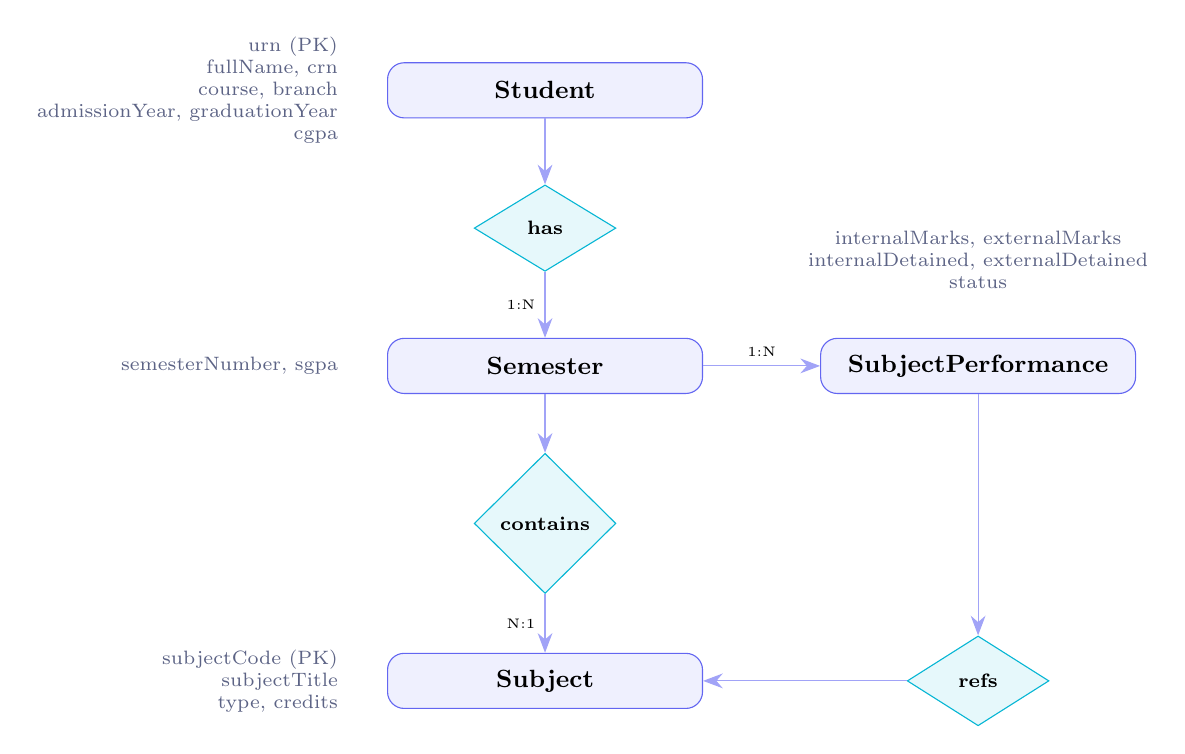
\begin{tikzpicture}[
  entity/.style={rectangle, draw=primaryblue, fill=primaryblue!10, rounded corners=6pt, minimum width=4cm, minimum height=0.7cm, align=center, font=\small\bfseries},
  attr/.style={font=\scriptsize, text=textmuted},
  rel/.style={diamond, draw=accentcyan, fill=accentcyan!10, minimum width=1.8cm, minimum height=1cm, align=center, font=\scriptsize\bfseries},
  arrow/.style={-{Stealth[length=2.5mm]}, draw=primaryblue!60}
]
  % Entities
  \node[entity] (student) at (0, 0) {Student};
  \node[entity] (semester) at (0, -3.5) {Semester};
  \node[entity] (subject) at (0, -7.5) {Subject};
  \node[entity] (performance) at (5.5, -3.5) {SubjectPerformance};

  % Relationships
  \node[rel] (r1) at (0, -1.75) {has};
  \node[rel] (r2) at (0, -5.5) {contains};
  \node[rel] (r3) at (5.5, -7.5) {refs};

  % Attributes
  \node[attr, left=0.5cm of student, align=right] {urn (PK)\\fullName, crn\\course, branch\\admissionYear, graduationYear\\cgpa};
  
  \node[attr, left=0.5cm of semester, align=right] {semesterNumber, sgpa};
  
  \node[attr, left=0.5cm of subject, align=right] {subjectCode (PK)\\subjectTitle\\type, credits};
  
  \node[attr, above=0.5cm of performance, align=center] {internalMarks, externalMarks\\internalDetained, externalDetained\\status};

  % Arrows
  \draw[arrow] (student) -- (r1);
  \draw[arrow] (r1) -- node[left, font=\tiny] {1:N} (semester);
  
  \draw[arrow] (semester) -- (r2);
  \draw[arrow] (r2) -- node[left, font=\tiny] {N:1} (subject);
  
  \draw[arrow] (performance) -- (r3);
  \draw[arrow] (r3) -- (subject);
  
  \draw[arrow] (semester) -- node[above, font=\tiny] {1:N} (performance);
\end{tikzpicture}
\caption{Entity-Relationship Diagram}
\end{figure}

The Entity-Relationship (ER) Diagram (Figure 4.7) models the core data structures and their associations within the database. A single Student entity has multiple Semester entities (1:N), and each Semester contains multiple SubjectPerformance records (1:N). Each SubjectPerformance record references a specific Subject. The physical layout separates overlapping attributes to distinctly list unique identifiers like the URN for students and subjectCode for subjects.

\subsection{Database Schema Details}

\textbf{Student Collection:}
\begin{longtable}{|l|l|p{10cm}|}
\hline
\textbf{Field} & \textbf{Type} & \textbf{Description}\\
\hline
fullName & String & Student's full name (required, trimmed)\\
\hline
urn & Number & University Roll Number (unique, required)\\
\hline
crn & Number & Class Roll Number (required)\\
\hline
course & String & Course enrolled (validated against courseBranchMap)\\
\hline
branch & String & Branch of study (validated per course)\\
\hline
admissionYear & Number & Year of admission (min: 2000)\\
\hline
graduationYear & Number & Expected graduation year ($>$ admissionYear)\\
\hline
semesters & Array & Array of Semester sub-documents\\
\hline
guardianEmail & String & Parent/Guardian email for notifications\\
\hline
cgpa & Number & Auto-calculated \textbf{only after degree completion}\\
\hline
\end{longtable}

\textbf{Subject Collection:}
\begin{longtable}{|l|l|p{8cm}|}
\hline
\textbf{Field} & \textbf{Type} & \textbf{Description}\\
\hline
subjectCode & String & Unique code (uppercase, trimmed)\\
\hline
subjectTitle & String & Full subject name\\
\hline
type & String & ``T'' (Theory) or ``P'' (Practical)\\
\hline
credits & Number & Credit weight of the subject\\
\hline
maxInternalMarks & Number & Maximum internal marks\\
\hline
maxExternalMarks & Number & Maximum external marks\\
\hline
maxTotalMarks & Number & $\geq$ maxInternal + maxExternal\\
\hline
minInternalPassMarks & Number & Minimum to pass internally\\
\hline
minExternalPassMarks & Number & Minimum to pass externally\\
\hline
minTotalPassMarks & Number & $\leq$ maxTotalMarks\\
\hline
\end{longtable}

\textbf{Token Collection:}
\begin{longtable}{|l|l|p{8cm}|}
\hline
\textbf{Field} & \textbf{Type} & \textbf{Description}\\
\hline
student & ObjectId & Reference to the Student document\\
\hline
token & String & Unique cryptographically secure token string\\
\hline
semester & Number & The academic semester for this report\\
\hline
sentVia & String & Delivery method (Email, SMS, Both)\\
\hline
expiresAt & Date & Timestamp after which the token is invalid\\
\hline
isRevoked & Boolean & Manual override to invalidate token access\\
\hline
\end{longtable}

\section{Component Diagram -- Frontend Architecture}

\begin{figure}[H]
\centering
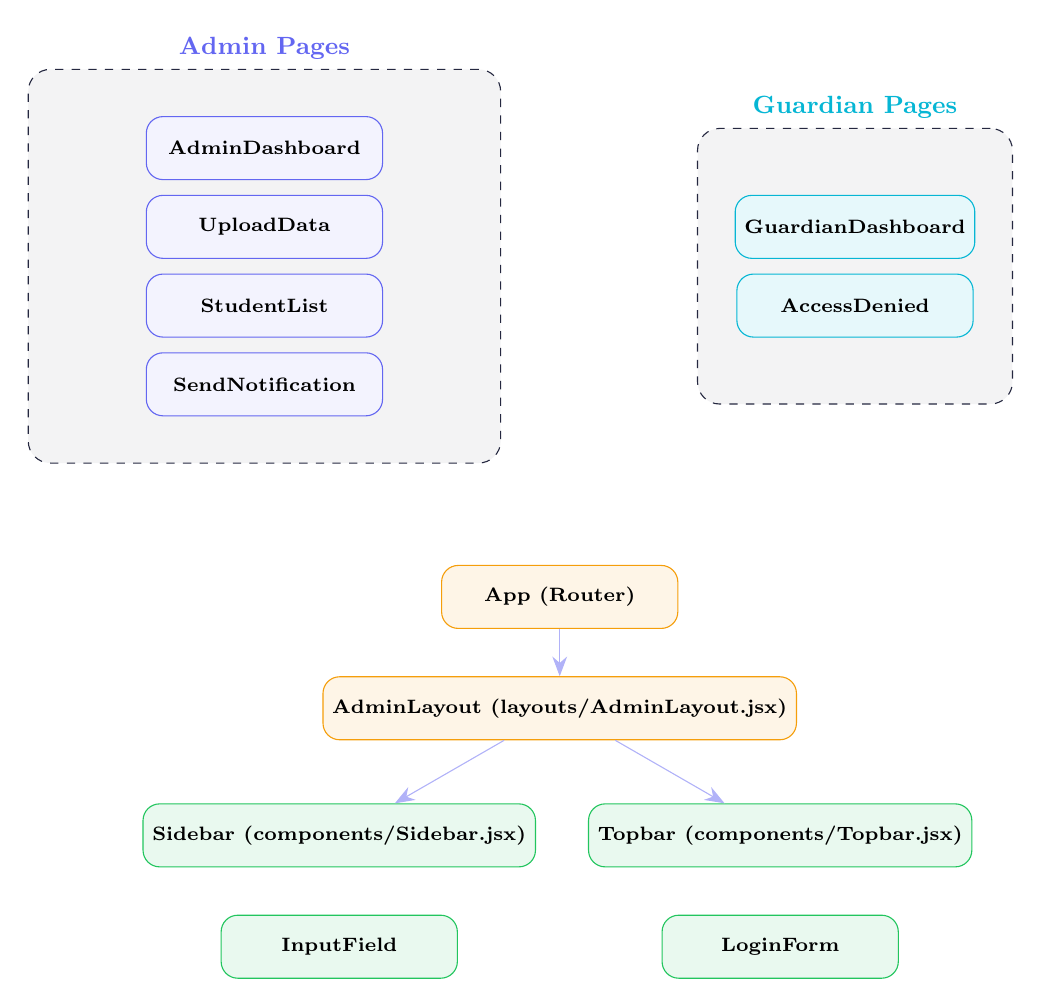
\begin{tikzpicture}[
  comp/.style={rectangle, draw=primaryblue, fill=primaryblue!8, rounded corners=6pt, minimum width=3cm, minimum height=0.8cm, align=center, font=\scriptsize\bfseries},
  pkg/.style={rectangle, draw=bordercolor, dashed, rounded corners=8pt, inner sep=10pt, fill=cardbg!5},
  arrow/.style={-{Stealth[length=2.5mm]}, draw=primaryblue!50}
]
  % Packages
  \node[pkg, minimum width=6cm, minimum height=5cm, label={[font=\small\bfseries, text=primaryblue]above:Admin Pages}] (adminpkg) at (-3.5, -0.3) {};
  \node[pkg, minimum width=4cm, minimum height=3.5cm, label={[font=\small\bfseries, text=accentcyan]above:Guardian Pages}] (guardpkg) at (4, -0.3) {};

  % Admin components
  \node[comp] (adash) at (-3.5, 1.2) {AdminDashboard};
  \node[comp] (aupload) at (-3.5, 0.2) {UploadData};
  \node[comp] (alist) at (-3.5, -0.8) {StudentList};
  \node[comp] (anotify) at (-3.5, -1.8) {SendNotification};

  % Guardian components
  \node[comp, fill=accentcyan!10, draw=accentcyan] (gdash) at (4, 0.2) {GuardianDashboard};
  \node[comp, fill=accentcyan!10, draw=accentcyan] (gaccess) at (4, -0.8) {AccessDenied};

  % Layout
  \node[comp, fill=warningamber!10, draw=warningamber] (router) at (0.25, -4.5) {App (Router)};
  \node[comp, below=0.6cm of router, fill=warningamber!10, draw=warningamber] (layout) {AdminLayout (layouts/AdminLayout.jsx)};

  % Shared
  \node[comp, below=0.8cm of layout, xshift=-2.8cm, fill=successgreen!10, draw=successgreen] (sidebar) {Sidebar (components/Sidebar.jsx)};
  \node[comp, below=0.8cm of layout, xshift=2.8cm, fill=successgreen!10, draw=successgreen] (topbar) {Topbar (components/Topbar.jsx)};
  \node[comp, below=0.6cm of sidebar, fill=successgreen!10, draw=successgreen] (input) {InputField};
  \node[comp, below=0.6cm of topbar, fill=successgreen!10, draw=successgreen] (loginform) {LoginForm};

  \draw[arrow] (router) -- (layout);
  \draw[arrow] (layout) -- (sidebar);
  \draw[arrow] (layout) -- (topbar);
\end{tikzpicture}
\caption{Frontend Component Architecture}
\end{figure}

The Frontend Component Architecture (Figure 4.8) showcases the modular design of the React application. It separates components into logically grouped packages: Admin Pages (e.g., Dashboard, Upload Data, Student List) and Guardian Pages (e.g., Guardian Dashboard, Access Denied). Shared UI components like the Sidebar, Topbar, and Input Fields are reused across different layouts. The root App Router strictly manages navigation dynamically routing users depending on their access role.

\section{Deployment Diagram}

\begin{figure}[H]
\centering
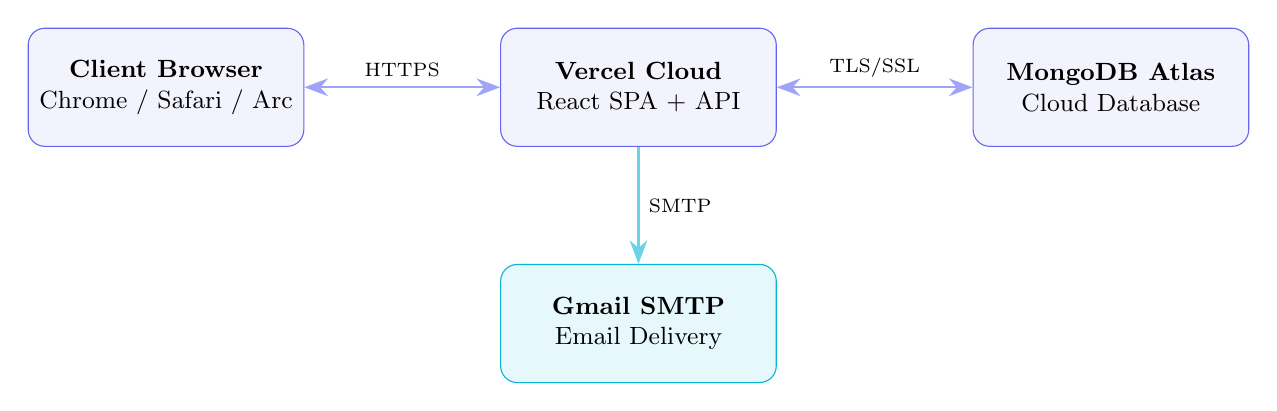
\begin{tikzpicture}[
  node3d/.style={rectangle, draw=primaryblue, fill=primaryblue!8, rounded corners=6pt, minimum width=3.5cm, minimum height=1.5cm, align=center, font=\small},
  arrow/.style={{Stealth[length=3mm]}-{Stealth[length=3mm]}, thick, draw=primaryblue!60}
]
  \node[node3d] (client) at (0, 0) {\textbf{Client Browser}\\Chrome / Safari / Arc};
  \node[node3d] (vercel) at (6, 0) {\textbf{Vercel Cloud}\\React SPA + API};
  \node[node3d] (atlas) at (12, 0) {\textbf{MongoDB Atlas}\\Cloud Database};
  \node[node3d, fill=accentcyan!10, draw=accentcyan] (gmail) at (6, -3) {\textbf{Gmail SMTP}\\Email Delivery};

  \draw[arrow] (client) -- node[above, font=\scriptsize] {HTTPS} (vercel);
  \draw[arrow] (vercel) -- node[above, font=\scriptsize] {TLS/SSL} (atlas);
  \draw[-{Stealth[length=3mm]}, thick, draw=accentcyan!60] (vercel) -- node[right, font=\scriptsize] {SMTP} (gmail);
\end{tikzpicture}
\caption{Deployment Diagram}
\end{figure}

The Deployment Diagram (Figure 4.9) depicts the physical architecture and network interactions of the production system. Client browsers communicate securely via HTTPS with the Vercel Cloud, which hosts the React Single Page Application (SPA) and backend serverless API functions. In turn, the Vercel infrastructure connects to the MongoDB Atlas cluster over TLS/SSL for database operations and interacts with the Gmail SMTP server to handle outbound email delivery.

\section{State Diagram}

\begin{figure}[H]
\centering
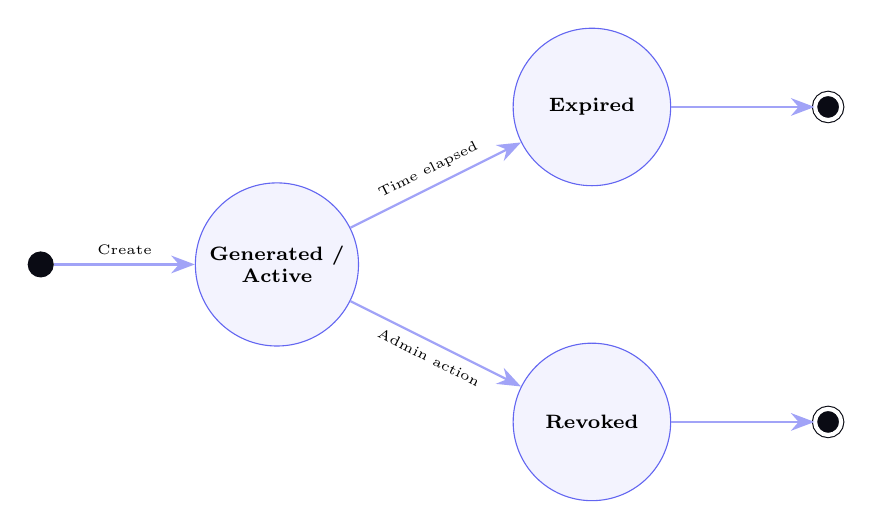
\begin{tikzpicture}[
  state/.style={circle, draw=primaryblue, fill=primaryblue!8, minimum size=2cm, align=center, font=\scriptsize\bfseries},
  initial/.style={circle, fill=darkbg, minimum size=0.3cm},
  final/.style={circle, draw=darkbg, fill=darkbg, minimum size=0.3cm, double, double distance=1.5pt},
  arrow/.style={-{Stealth[length=3mm]}, thick, draw=primaryblue!60}
]
  \node[initial] (start) at (0, 0) {};
  \node[state] (generated) at (3, 0) {Generated /\\Active};
  \node[state] (expired) at (7, 2) {Expired};
  \node[state] (revoked) at (7, -2) {Revoked};
  \node[final] (end_exp) at (10, 2) {};
  \node[final] (end_rev) at (10, -2) {};

  \draw[arrow] (start) -- node[above, font=\tiny] {Create} (generated);
  \draw[arrow] (generated) -- node[above, font=\tiny, sloped] {Time elapsed} (expired);
  \draw[arrow] (generated) -- node[below, font=\tiny, sloped] {Admin action} (revoked);
  \draw[arrow] (expired) -- (end_exp);
  \draw[arrow] (revoked) -- (end_rev);
\end{tikzpicture}
\caption{State Machine Diagram -- Token Lifecycle}
\end{figure}

The State Diagram (Figure 4.10) illustrates the lifecycle and various states of an access token within the notification system. A token begins in the `Generated / Active' state immediately after dispatch. It transitions to an `Expired' state automatically after a predefined time limit, or to a `Revoked' state if an Admin manually invalidates it. Both Expired and Revoked act as terminal states where the token can no longer be used for Guardian authentication.

\section{Communication Diagram}

\begin{figure}[H]
\centering
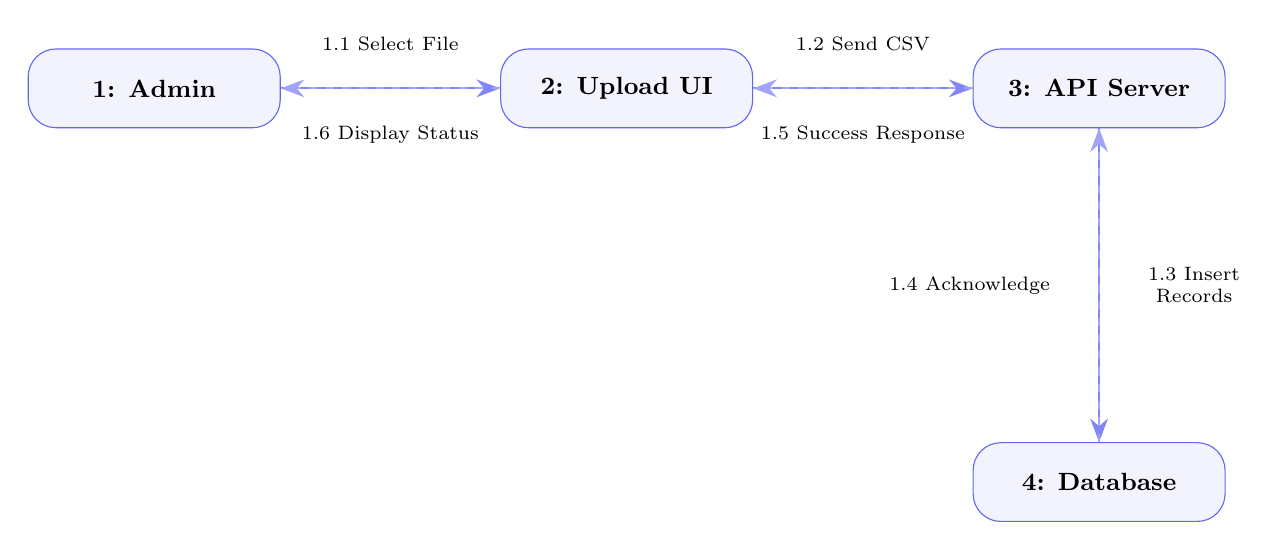
\begin{tikzpicture}[
  actor/.style={
    rectangle,
    draw=primaryblue,
    fill=primaryblue!8,
    rounded corners=10pt,
    minimum width=3.2cm,
    minimum height=1cm,
    align=center,
    font=\small\bfseries,
    inner sep=8pt
  },
  req/.style={
    -{Stealth[length=3mm]},
    thick,
    draw=primaryblue!80
  },
  res/.style={
    -{Stealth[length=3mm]},
    thick,
    dashed,
    draw=primaryblue!60
  }
]

% Nodes (better horizontal spacing)
\node[actor] (admin)   at (0,0)   {1: Admin};
\node[actor] (ui)      at (6,0)   {2: Upload UI};
\node[actor] (backend) at (12,0)  {3: API Server};
\node[actor] (db)      at (12,-5) {4: Database};

% Forward Flow
\draw[req] (admin) -- 
node[midway, above=10pt, font=\scriptsize] {1.1 Select File}
(ui);

\draw[req] (ui) -- 
node[midway, above=10pt, font=\scriptsize] {1.2 Send CSV}
(backend);

\draw[req] (backend) -- 
node[midway, right=14pt, font=\scriptsize, align=center] 
{1.3 Insert\\Records}
(db);

% Response Flow (dashed for clarity)
\draw[res] (db) -- 
node[midway, left=14pt, font=\scriptsize] 
{1.4 Acknowledge}
(backend);

\draw[res] (backend) -- 
node[midway, below=10pt, font=\scriptsize] 
{1.5 Success Response}
(ui);

\draw[res] (ui) -- 
node[midway, below=10pt, font=\scriptsize] 
{1.6 Display Status}
(admin);

\end{tikzpicture}
\caption{Communication Diagram -- Bulk Data Upload}
\end{figure}

The Communication Diagram (Figure 4.11) models the dynamic behavior and message flows during the bulk data upload process. Unlike a Sequence Diagram, it emphasizes the structural relationships between objects. The interaction begins with the Admin selecting a file in the Upload UI (1.1). The UI then transmits the parsed CSV data to the API Server (1.2), which inserts the records into the Database (1.3). The sequence elegantly wraps up as acknowledgments flow back from the Database through the API Server to update the UI on the operation's success.

%% ===========================
%% CHAPTER 5: TESTING MODULE
%% ===========================
\chapter{Testing Module}

\section{Proposed Testing Approach}

As the system is currently under development, this section outlines the proposed testing techniques that will be employed to ensure the robustness, reliability, and functionality of the Academic Status Transparency Notification System (ASTNS). The system will undergo testing using a combination of manual functional testing, automated unit testing, API integration testing, and cross-browser validation.

The proposed testing strategy will cover:

\begin{enumerate}
  \item \textbf{Unit-Level Validation}: Validating individual components such as Mongoose schema validators (e.g., marks ranges, course-branch mapping, CGPA calculation constraints).
  \item \textbf{API Integration Testing}: Testing the REST API endpoints using tools like Postman or Thunder Client to ensure correct request handling and response payloads.
  \item \textbf{UI/UX Functional Testing}: Performing manual browser testing on Google Chrome, Apple Safari, and Arc for cross-browser parity and user experience.
  \item \textbf{Cross-Device Verification}: Verifying the responsive layout on desktop, tablet, and mobile viewports.
  \item \textbf{Email Delivery Testing}: Simulating notification dispatch to verify Gmail SMTP delivery capabilities, HTML template rendering, and dynamic link mapping.
\end{enumerate}

\section{Proposed Test Cases}

The following is a curated list of relevant test cases on which the system will be systematically tested during the verification phase.

\begin{longtable}{|p{1cm}|p{3cm}|p{5cm}|p{5cm}|}
\hline
\textbf{ID} & \textbf{Test Case} & \textbf{Steps} & \textbf{Expected Outcome}\\
\hline
\endfirsthead
\hline
\textbf{ID} & \textbf{Test Case} & \textbf{Steps} & \textbf{Expected Outcome}\\
\hline
\endhead
TC1 & Admin Login -- Valid & Enter assigned admin credentials, click Submit & Successful redirection to Admin Dashboard\\
\hline
TC2 & Admin Login -- Invalid & Enter wrong credentials, click Submit & Appropriate error message displayed\\
\hline
TC3 & Login Form Validation & Attempt to submit an empty or incomplete login form & Required field validation errors shown\\
\hline
TC4 & Email Regex Validation & Enter malformed or non-Gmail email address & Appropriate pattern constraint error shown\\
\hline
TC5 & Bulk CSV Upload & Upload a correctly formatted CSV/Excel data file & Academic records parsed and previewed correctly\\
\hline
TC6 & Invalid File Upload & Attempt to upload unsupported file type (e.g., .txt) & File rejection with corresponding error alert\\
\hline
TC7 & Student Search Filtering & Input part of a student name in the search bar & List filtered down to match search string dynamically\\
\hline
TC8 & View Student Profile & Click on a specific student record card & Detailed profile page with accurate academic charts loads\\
\hline
TC9 & Batch Notification Dispatch & Select multiple students and trigger Send Notification & Successful API execution with UI confirmation message\\
\hline
TC10 & Guardian Token Validation & Access Guardian Portal via uniquely generated token link & Student semester report accurately displayed for authorized token\\
\hline
TC11 & Invalid Token Handling & Attempt accessing portal with expired or altered token & Access Denied interface shown instead of reports\\
\hline
TC12 & Token Revocation Process & Admin clicks Revoke for an active token in dashboard & Token status instantly updates to Revoked across system\\
\hline
TC13 & SGPA Chart Rendering & Open student detail page containing multiple semesters & Multi-node line chart dynamically renders correct SGPA trend\\
\hline
TC14 & Responsive Layout Check & Resize browser window to mobile width ($< 768$px) & Layout reflows correctly, sidebar collapses into hamburger menu\\
\hline
TC15 & Email Template Rendering & Guardian receives dispatched notification email & Branded HTML email loads properly with clickable CTA button\\
\hline
\end{longtable}

%% ===========================
%% CHAPTER 6: CURRENT PROJECT STATUS
%% ===========================
\chapter{Performance of the Project Developed}

\section{Development Progress and Milestones}

As of the midterm evaluation, the core foundational architecture of the Academic Status Transparency Notification System (ASTNS) has been established. Our primary focus thus far has been to secure the backend infrastructure and prepare the frontend layout necessary for data ingestion and user interaction.

The following modules have been substantially developed and are currently undergoing internal testing:

\begin{itemize}
  \item \textbf{Authentication Module}: Admin login interface with robust \textbf{Axios}-based session management and route protection is functional.
  \item \textbf{Database Schema}: Mongoose models for Students, Semesters, Subjects, Performance, and \textbf{Secure Tokens} have been deployed to MongoDB Atlas.
  \item \textbf{Frontend Layouts}: The overarching React application architecture is fully integrated using Tailwind CSS, featuring a responsive Sidebar with logout confirmation.
  \item \textbf{Automated Email Notification Pipeline}: Integration with Gmail SMTP via Nodemailer for batch notification dispatch is operational.
  \item \textbf{Secure Token Generation System}: Cryptographic token generation and lifecycle management (expiry/revocation) are fully implemented.
\end{itemize}

\section{Remaining Requirements for Finalization}

To transition the project from its current midterm state to a fully finalized application, several critical features and integrations must be completed:

\begin{enumerate}
  \item \textbf{Robust Bulk Data Processing Integration}: Finalising the UI-to-Backend mapping for all student fields (including guardian emails) across complex multi-semester datasets.
  \item \textbf{Data Visualization Polishing}: Enhancing Recharts integration to provide even more granular academic insights on the Guardian Dashboard.
  \item \textbf{Comprehensive Role-Based Access Control Audit}: Performing a final security audit on server-side validations to ensure absolute data isolation.
  \item \textbf{Production Deployment}: Finalising Vercel production environment configurations and custom domain mapping.
\end{enumerate}

\section{Anticipated Ongoing Challenges}

During the subsequent development phases, We anticipate the following technical challenges that will require mitigation:

\begin{itemize}
  \item \textbf{Performance at Scale}: Ensuring the database querying and frontend rendering remain performant when simultaneously loading hundreds of detailed student profiles.
  \item \textbf{Email Delivery Reliability}: Guaranteeing that automated midterm and end-semester notifications bypass strict parental spam filters and bounce-backs are handled gracefully.
  \item \textbf{Asynchronous Error Handling}: Providing clear, actionable error messages to the administrator if a batch upload fails partially (e.g., if 5 out of 100 rows in a CSV are corrupted) rather than failing the entire process silently.
\end{itemize}

%% ===========================
%% CHAPTER 7: OUTPUT SCREENS
%% ===========================
\chapter{Output Screens}

\vspace{1cm}

\begin{enumerate}
  \item \textbf{Login Page} -- Dark-themed admin login with email/password fields, React Hook Form validation, gradient logo, and grid background.
  
  \begin{figure}[H]
  \centering
  \includegraphics[width=0.6\textwidth]{assets/pic1.png}
  \caption{Login Page}
  \end{figure}  

  \item \textbf{Admin Dashboard} -- Stat cards (Total Students, Notifications Sent, Detained, Active Tokens, Average CGPA), Area chart for notification activity, Bar chart for branch distribution, Recent uploads table.

  \begin{figure}[H]
  \centering
  \includegraphics[width=0.9\textwidth]{assets/pic2.png}
  \caption{Admin Dashboard}
  \end{figure} 

  \item \textbf{Upload Data} -- Course/branch/semester selection dropdowns, drag-and-drop CSV/Excel upload zone, parsed data preview table.

  \begin{figure}[H]
  \centering
  \includegraphics[width=0.9\textwidth]{assets/pic3.png}
  \caption{Upload Data}
  \end{figure} 

  \item \textbf{Student List} -- Searchable grid/list view with SGPA colour coding, branch filter, click-to-navigate to detail.

  \begin{figure}[H]
  \centering
  \includegraphics[width=0.9\textwidth]{assets/pic4.png}
  \caption{Student List}
  \end{figure} 

  \item \textbf{Student Detail} -- Student profile header, SGPA trend line chart, semester-wise collapsible tables showing internal/external marks and detention flags.

  \begin{figure}[H]
  \centering
  \includegraphics[width=0.9\textwidth]{assets/pic5.png}
  \caption{Student Detail}
  \end{figure} 

  \item \textbf{Send Notification} -- Multi-select student table, dispatch button with success/failure feedback.

  \begin{figure}[H]
  \centering
  \includegraphics[width=0.9\textwidth]{assets/pic6.png}
  \caption{Send Notification}
  \end{figure} 

  \item \textbf{Token Management} -- Token table with status badges (Active/Expired/Revoked), access method tags, revoke and copy-link actions.
  
  \begin{figure}[H]
  \centering
  \includegraphics[width=0.9\textwidth]{assets/pic7.png}
  \caption{Token Management}
  \end{figure} 

  \item \textbf{Guardian Dashboard} -- Token-authenticated view with student summary, SGPA chart, semester breakdown tables, attendance ring, and download report button.
  
  \begin{figure}[H]
  \centering
  \includegraphics[width=0.9\textwidth]{assets/pic8.png}
  \caption{Guardian Dashboard}
  \end{figure} 

  \begin{figure}[H]
  \centering
  \includegraphics[width=0.9\textwidth]{assets/pic9.png}
  \caption{Guardian Dashboard}
  \end{figure} 

  \item \textbf{Access Denied Page} -- Shown when token is invalid/expired/revoked.
  
  \begin{figure}[H]
  \centering
  \includegraphics[width=0.9\textwidth]{assets/pic10.png}
  \caption{Access Denied Page}
  \end{figure} 

  \item \textbf{Email Template} -- Branded HTML email with ``View Report'' CTA button.
  
  \begin{figure}[H]
  \centering
  \includegraphics[width=1\textwidth]{assets/pic11.png}
  \caption{Email Template}
  \end{figure} 

\end{enumerate}

%% ===========================
%% CHAPTER 8: REFERENCES
%% ===========================
\chapter{References}

\begin{enumerate}
  \item React Documentation -- \url{https://react.dev/}
  \item Express.js v5 Documentation -- \url{https://expressjs.com/}
  \item MongoDB Documentation -- \url{https://www.mongodb.com/docs/}
  \item Mongoose ODM Documentation -- \url{https://mongoosejs.com/docs/}
  \item Nodemailer Documentation -- \url{https://nodemailer.com/}
  \item Tailwind CSS v4 Documentation -- \url{https://tailwindcss.com/docs}
  \item Recharts Documentation -- \url{https://recharts.org/en-US/}
  \item React Hook Form Documentation -- \url{https://react-hook-form.com/}
  \item Vite Build Tool -- \url{https://vitejs.dev/}
  \item Lucide Icons -- \url{https://lucide.dev/}
  \item Vercel Deployment Platform -- \url{https://vercel.com/docs}
  \item React Router v7 -- \url{https://reactrouter.com/}
  \item Minor Project Synopsis -- Group G14, Department of CSE, GNDEC Ludhiana.
\end{enumerate}

\end{document}
